\documentclass{warpdoc}
\newlength\lengthfigure                  % declare a figure width unit
\setlength\lengthfigure{0.158\textwidth} % make the figure width unit scale with the textwidth
\usepackage{psfrag}         % use it to substitute a string in a eps figure
\usepackage{subfigure}
\usepackage{rotating}
\usepackage{pstricks}
\usepackage[innercaption]{sidecap} % the cute space-saving side captions
\usepackage{scalefnt}
\usepackage{amsbsy}
\usepackage{bm}
\usepackage{amsmath}
\usepackage{array}
%\usepackage{kpfonts}
\usepackage{float}
\usepackage{caption}
%%%%%%%%%%%%%=--NEW COMMANDS BEGINS--=%%%%%%%%%%%%%%%%%%%%%%%%%%%%%%%%%%
\newcommand{\alb}{\vspace{0.2cm}\\} % array line break
\newcommand{\mfd}{\displaystyle}
\renewcommand{\fontsizetable}{\footnotesize\scalefont{0.7}}
\renewcommand{\fontsizefigure}{\footnotesize}
\newcommand{\Bdipole}{B_{\rm d}}
\newcommand{\ns}{{n_{\rm s}}}
\newcommand\frameeqn[1]{\fbox{$\displaystyle #1$}}
\newcommand\framealign[1]{\fbox{\begin{align}#1\end{align}}}
\newcommand{\nd}{3}

\renewcommand{\vec}[1]{\bm{#1}}

\setcounter{tocdepth}{3}

\let\citen\cite

%%%%%%%%%%%%%=--NEW COMMANDS BEGINS--=%%%%%%%%%%%%%%%%%%%%%%%%%%%%%%%%%%

\setcounter{tocdepth}{3}

%%%%%%%%%%%%%=--NEW COMMANDS ENDS--=%%%%%%%%%%%%%%%%%%%%%%%%%%%%%%%%%%%%



\author{
  Vasilis Tsakagiannis
}

\email{
  vtsakag@gmail.com
}

\department{
  Aerospace and Mechanical Engineering
}

\institution{
  University of Arizona
}

\title{
  Radiation Heat Transfer Hydrodynamic Model  
}

\date{
  2019
}

%\setlength\nomenclaturelabelwidth{0.13\hsize}  % optional, default is 0.03\hsize
%\setlength\nomenclaturecolumnsep{0.09\hsize}  % optional, default is 0.06\hsize

\nomenclature{

  \begin{nomenclaturelist}{Roman symbols}
   \item[$\Vec{s}$] direction vector of the intensity, m
   \item[$\Vec{x}$] position vector on the flow field, m
   \item[$I$] radiation intensity, W/$\text{m}^2$ster
   \item[$B$] emission source term, W/$\text{m}^2$ster
   
   \item[$\Vec{\dot{q}_{\text{rad}}}$] radiant heat flux vector, W/$\text{m}^2$
   \item[$U_{\text{rad}}$] local incident radiation intensity, W/$\text{m}^2$
   \item[$N_{\Omega}$] number of control angles
   \item[$\phi$] azimuthal angle, rad
   \item[$\theta$] polar angle, rad
   \item[$\delta \Omega$] solid angle, ster
   \item[$N_\text{B}$] number of spectral bands
   \item[$C_2$] Planck's second radiation constant, mK
   \item[$\lambda_{{\text{min/max}}}$] lower/upper boundary of the wavelength of the band, m
   \item[$Z_\text{min/max}$] quantity used for the calculation of the correction term
   \item[$F_\text{min/max}$] quantity used for the calculation of the correction term
   \item[$F_\text{N}$] correction term
   \item[$\Vec{s_{\text{x}}}$] $x$ component of the direction vector of the intensity, m
   \item[$k_\text{abs}$] Planck mean absorption coefficient, 1/m
   \item[$I_\text{b}$] intensity radiation from the source term, W/$\text{m}^2$ster
   \item[$d\text{x}$] distance between two adjacent nodes, m
   \item[$l$] length of the domain, m
   \item[$y$] mol fraction
   \item[$I_\text{face}$] radiation intensity at the face of the cell, W/$\text{m}^2$ster
   \item[$Q_\text{rad}$] radiative loss term, W/$\text{m}^3$
   \item[$U$] flow velocity, m/s
   \item[$r$] radius, m
   \item[$t$] time, s
   \item[$m$] mass, kg
   \item[$p$] pressure, Pa
   
   \item[$p_0$] undisturbed air pressure, Pa
   
   \item[$Y$] artificial viscosity
   \item[$Q$] influx and heat losses, W/$\text{m}^3$
   
   \item[$Q_\text{J}$] joule heating, W/$\text{m}^3$
   
  % \item[$Q_{\lambda}$] radiation losses, W/$\text{m}^3$
   
  % \item[$Q_{rad}$] heat conductivity, W/$\text{m}^3$
   
   \item[$h$] specific enthalpy, J/kg
   \item[$T$] temperature, K
   \item[$E$] electric field, V/m
 %  \item[$I$] current pulse, A
   \item[$v$] frequency, Hz
   \item[$I_\text{a}$] amplitude of aperiodic current pulse, A
   \item[$\tau_\text{a}$] characteristic decay time, s
   \item[$I_\text{res}$] residual after discharge, A
   \item[$R$] channel resistance per unit length, ${\Omega}$/m
   
   \item[$A_0$] fraction of air molecules dissociated to atoms
   
   \item[$A_1$] fraction of ionized atoms
   
   \item[$A_2$] fraction of single ions which have lost a second electron
   \item[$a_\text{iav}$] average electron ion cross section
  \item[$k$] thermal conductivity coefficient of air, W/mK
   \item[$k_\text{e}$] thermal conductivity coefficient  by electrons,W/mK
   \item[$k_\text{r}$] diffusion of recombination energy coefficient, W/mK
   \item[$k_0$] thermal conductivity coefficient by neutral particles, W/mK

   
   \item[$c$] velocity of light, m/s
   
  % \item[$h$] Planck's constant, Js
   
  % \item[$B$] Planck's radiation expression for blackbody, W/$\text{m}^2$
   
   \item[$k_\text{B}$] Boltzman's constant, J/K
   
   %\item[$k_v$] absorption coefficient, 1/m
   
  % \item[E] Energy of the electromagnetic spectrum, eV
   
   \item[$U_\text{v}$] spectral density of radiation power, $\text{W}^2/\text{m}^6$Hz
   
   \item[$U_\text{pv}$] spectral density of radiation power at equilibrium,  $\text{W}^2/\text{m}^6$Hz
   
   
   \end{nomenclaturelist}

  \begin{nomenclaturelist}{Greek symbols}
     
  
     \item[$\rho$] density, kg/$\text{m}^3$
   
    \item[$\rho_0$] undisturbed air density, kg/$\text{m}^3$
   
     \item[$\epsilon$] specific internal energy, J/kg
   
     \item[$\gamma$] specific heat ratio
   
  %   \item[$\sigma$] conductivity of plasma, S/m
     
     \item[$\sigma$] Stefan-Boltzmann constant, W/$\text{m}^2\text{K}^4$
     
     \item[$\lambda$] wavelength of the electromagnetic radiation, m
     \item[$\kappa$] absorption coefficient, 1/m
  \end{nomenclaturelist}
}
 

\abstract{
In the present work, the one dimensional radiation equation is solved numerically in order to be further generalised in three dimensions so it can be implemented in CFDWARP. The main purpose of the model presented here, is to simulate the radiative heat transfer effects on a flow field. On this document two different formulations of the radiation  equation are presented. The specific model accompanied with some modifications can be useful for simulating cases such as re-entry flows and lightning strike on a structure.    
}

\begin{document}

  \pagestyle{headings}
  \pagenumbering{arabic}
  \setcounter{page}{1}
%%  \maketitle
  \makewarpdoctitle
  \makeabstract
  \tableofcontents

  \makenomenclature

%\printnomenclature
%%  \listoftables
%%  \listoffigures



\section{Fluid Convection Model for Radiation Heat Transfer}
\subsection{Presentation of the Equation}
The radiative heat transfer phenomena for an absorbing and emitting medium, can be described by the Eq. \eqref{eq:rte1}, which is called Radiative Transport equation (RTE).
\begin{equation}
    \Vec{s}\cdot \nabla I(\Vec{x},\Vec{s},\lambda)=B(\Vec{x},\lambda)-\kappa(\Vec{x},\lambda)I(\Vec{x},\Vec{s},\lambda)
    \label{eq:rte1}
\end{equation}
Here, $\Vec{x}$ is the position vector on the flow field, $\Vec{s}$ is the direction vector of the radiation intensity, $I(\Vec{x},\Vec{s},\lambda)$ is the radiation intensity of the flow filed at $\Vec{x}$, at wavelength $\lambda$ and with the direction of $\Vec{s}$. Finally $B(\Vec{x},\lambda)$ is the emission source term, which is modeled with the radiation emitted by the blackbody, and is describe by Eq. \eqref{eq:source1}
\begin{equation}
    B(\Vec{x},\lambda)=\kappa(\Vec{x},\lambda)I_\text{b}(\Vec{x},\lambda)=\kappa(\Vec{x},\lambda)\frac{\sigma T(\Vec{x})^4}{\pi}
    \label{eq:source1}
\end{equation}
where $I_\text{b}(\Vec{x},\lambda)$ is the radiation intensity because of the  the blackbody source term, $\sigma=5.67037\times 10^{-8}$  ${\text{W}/\text{m}^2\text{K}^4}$ is the Stefan-Boltzmann constant, and $T(\Vec{x})$ is the temperature of the fluid.
\\
We can calculate the radiant heat flux vector on the surface of a sphere of radius $r=1$ m from Eq. \eqref{eq:radflux} and define the local incident radiation intensity from Eq. \eqref{eq:incrad}.
\begin{equation}
    \Vec{\dot{q}_\text{rad}}(\Vec{x},\lambda)=\int_{4\pi}^{} \Vec{s}I(\Vec{x},\Vec{s},\lambda)d\Vec{s}
    \label{eq:radflux}
\end{equation}
\begin{equation}
    U_\text{rad}(\Vec{x},\lambda)=\int_{4\pi}^{} I(\Vec{x},\Vec{s},\lambda)d\Vec{s}
    \label{eq:incrad}
\end{equation}
If we integrate both parts and substitute the radiant heat flux vector and the local incident radiation intensity on Eq. \eqref{eq:rte1}, we can obtain Eq. \eqref{eq:rte2} which is a more convenient form for our work because the term -$\nabla \Vec{\dot{q}_\text{rad}}(\Vec{x},\lambda)$ is the radiative loss term in the energy equation we want to actually calculate.
\begin{equation}
     -\nabla \Vec{\dot{q}_\text{rad}}(\Vec{x},\lambda)=\kappa(\Vec{x},\lambda)[ U_\text{rad}(\Vec{x},\lambda)-4\pi I_\text{b}(\Vec{x},\lambda)]
    \label{eq:rte2}
\end{equation}

\subsection{Numerical Method}
In this subsection, the numerical process is described step by step in order to finally calculate the radiative loss term we need. The methods presented bellow follow the work of the developers of Fire Dynamics Simulator, which is a powerful tool able to simulate fires and also includes a model for radiative heat transfer. Their work is described extensively in Ref. \cite{fdstechnical}.
\subsubsection{Angular Discretization}
In order to obtain the discrete form of Eq. \eqref{eq:rte2} we have first to discretize the sphere of radius $r=1$ m into a finite number of solid angles, where the direction of the radiation intensity is take into account. In Fig. \ref{fig:ang}, the coordinate system we use for the angular discretiazation can be seen, along with the direction vector of the radiation intensity $\Vec{s}$, which is specified by the polar angle $\theta$ and the azimuthal angle $\phi$, and finally the solid angle which is created on the surface of the sphere. For the one dimensional model here, was chosen to discretize the sphere into sixty control angles $N_{\Omega}=60$. The upper and lower limit of the polar and azimuthal angle, are denoted by the superscript + and - respectively, and they can be calculated by the Eqs. \eqref{eq:angdisc}, \eqref{eq:angdisc2}

 \begin{equation}
    \phi_k^+=\frac{2\pi k}{N_{\Omega}}+\frac{\pi}{2},\enspace
    \phi_k^-=\frac{2\pi(k-1)}{N_{\Omega}}+\frac{\pi}{2} 
    \label{eq:angdisc}
 \end{equation}
 
 \begin{equation}
     \theta_k^+=\pi,\enspace \theta_k^-=0 \label{eq:angdisc2}
 \end{equation}
where the subscript $k$ denotes the control angle index and takes values in the interval $[1,N_{\Omega}]$. Finally, the solid angle $\delta{\Omega}_k$ can be calculated by Eq. \eqref{eq:solidang}.

\begin{equation}
    \delta{\Omega}_k=[\cos(\theta_k^-)-\cos(\theta_k^+)](\phi_k^+-\phi_k^-)
     \label{eq:solidang}
\end{equation}

\begin{figure}[!h]
\centering
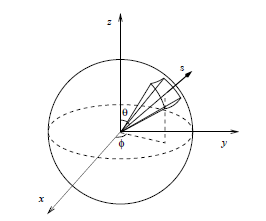
\includegraphics[width=0.45\textwidth]{angular_disc.png}
\caption{Coordinate system of the angular discretization}
\label{fig:ang}
\end{figure}
\subsubsection{Manipulation of the Radiant Spectrum}
The spectrum of the electromagnetic waves is continuous, and its wavelength ranges from nanometers to kilometers. In practical simulations it's impossible to model the whole spectrum because of the huge computational cost. In order to face this problem, in the present work the electromagnetic spectrum is divided into six bands $N_\text{B}=6$ where the discrete form of the RTE is solved separately. It's important to mention here that the absorption coefficient is taken directly from FDS for every cell and every band we solve for. 
\subsubsection{Spatial Discretization of the RTE}
The first step here is to impose the correct boundary conditions for the intensity radiation. The boundaries are treated as black walls, where the incoming radiation is the blackbody intensity of the ambient temperature. Here, we have to highlight that the present model uses a correction term for the blackbody intensity in order to obtain more realistic results, which is described in Ref. \cite{ref67}. This correction term is calculated by the following process 

\begin{equation} \begin{split} Z_{\min_{i,j}}=\frac{C_2}{\lambda_{{\min}_j}T_i} \\ Z_{\max_{i,j}}=\frac{C_2}{\lambda_{{\max}_j}T_i} \end{split} \label{eq:zita}\end{equation}
\begin{equation} \begin{split} F_{\min_{i,j}}=\frac{15}{\pi^4} \sum_{n=1}^{50} \frac{e^{-nZ_{\min_{i,j}}}}{n}(Z_{\min_{i,j}}^3+\frac{3Z_{\min_{i,j}}^2}{n}+\frac{6Z_{\min_{i,j}}}{n^2}+\frac{6}{n^3}) \\ F_{\max_{i,j}}=\frac{15}{\pi^4} \sum_{n=1}^{50} \frac{e^{-nZ_{\max_{i,j}}}}{n}(Z_{\max_{i,j}}^3+\frac{3Z_{\max_{i,j}}^2}{n}+\frac{6Z_{\max_{i,j}}}{n^2}+\frac{6}{n^3})  \end{split}\label{eq:FF} \end{equation}
\begin{equation} F_{\text{N}_{{i,j}}}=F_{\max_{i,j}}-F_{\min_{i,j}}\label{eq:Fn} \end{equation}
where $C_2=1.43877\times 10^{-2}$ mK is Planck's second radiation constant,$i$ is the cell index, $j$ is the band index taking values in the interval $[1,N_B]$, $\lambda_{{\min}_j}$ and $\lambda_{{\max}_j}$ are the lower and upper boundaries of the wavelength of each band, $T_i$ is the temperature of the cell, and finally $F_{\text{N}_{{i,j}}}$ is the correction term. The boundary conditions are implemented on the first an last cell of the computational domain are the following

\begin{equation} \begin{split} I_{1,j}=\frac{F_{\text{N}_{1,j}}}{\pi} \sigma T_1^4 \\ I_{N_x,j}=\frac{F_{\text{N}_{N_x,j}}}{\pi} \sigma T_{N_x}^4 \end{split} \end{equation}
where $N_x$ the number of the total nodes on the spatial discretization.\\
The next step is to solve for the unknown intensity radiation for every cell, every band of the spectrum and every direction. First, the direction vector of the radiation intensity of the x axis is discretized using Eq. \eqref{eq:sx1}.
\begin{equation} s_{\text{x}_k}=\cos\left(\phi_k^-+\frac{\phi_k^+-\phi_k^-}{2}\right)\sin\left(\theta_k^-+\frac{\theta_k^+-\theta_k^-}{2}\right) \label{eq:sx1}\end{equation}
For the spatial discretization of the RTE a first order upwind scheme is used, and the discrete form is shown in Eq. \eqref{eq:discrte}
\begin{equation}  I_{i,j,k}=\frac{k_{\text{abs}_{i,j}}I_{\text{b}_{i,j}} dx+|s_{\text{x}_k}|I_{\text{face}_{i,j,k}}}{|s_{\text{x}_k}|+k_{\text{abs}_{i,j}}dx} 
\label{eq:discrte} \end{equation}
where $k_{\text{abs}_{i,j}}$ is the Planck mean absorption coefficient for the $i^{th}$ cell and the $j^{th}$ band, $d\text{x}=\frac{l}{N_x-1}$ is the distance between two adjacent nodes, $l$ is the length of the domain, $I_{\text{b}_{i,j}}$ is the intensity radiation from the blackbody source term calculated from Eq. \eqref{eq:Ib} exactly the same way as the boundary conditions, and $I_{\text{face}_{i,j,k}}$ is the radiation intensity at the face of the cell calculated from Eq. \eqref{eq:face}. 

\begin{equation}
    I_{\text{b}_{i,j}}=\frac{F_{\text{N}_{i,j}}}{\pi} \sigma T_i^4
    \label{eq:Ib}
\end{equation}
\begin{equation}
    \begin{split}
       s_{\text{x}_k}>0,\enspace I_{\text{face}_{i,j,k}}=I_{i-1,j,k} \\ s_{\text{x}_k}<0,\enspace I_{\text{face}_{i,j,k}}=I_{i+1,j,k}
       \label{eq:face}
    \end{split}
\end{equation}
The final step is to calculate the radiative loss term from Eq. \eqref{eq:lossrad}
\begin{equation} Q_{\text{rad}_i}=\sum_{j=1}^{N_\text{B}} k_{\text{abs}_{i,j}}(U_{\text{rad}_{i,j}}-4\pi I_{\text{b}_{i,j}}) \label{eq:lossrad}\end{equation}
where  $U_{\text{rad}_{i,j}}$ is the local incident radiation intensity previously defined and can be calculated in discrete form form Eq. \eqref{eq:incrad2}.
\begin{equation} U_{\text{rad}_{i,j}}=\sum_{k=1}^{N_{\Omega}} I_{i,j,k}\delta  \Omega_k
\label{eq:incrad2}
\end{equation}

\subsubsection{Integration of the RTE}
In order to solve the discrete form of the RTE, an explicit spatial marching technique is used. The marching direction depends on the propagation direction of the radiation intensity and can be found by calculating $s_\text{x}$. While the marching is done on the downwind direction, the upwind intensities along with the intensities at the faces are all known, and the only unknowns are the downwind intensities, which can be found by the algebraic Eq. \eqref{eq:discrte}. For each cell in the domain, the intensity is calculated for each direction dependent from $s_{\text{x}}$ and for each spectral band. In other words, there are 60 marching sweeps per band and there are also 6 bands, meaning that the total number of marching sweeps per spatial iteration is equal to 360. For a three dimensional case, we would need 100 marching sweeps per band and the total number of marching sweeps per spatial iteration would be 600.
\subsection{Validation of the Code}
For the validation of the code the results of Fire Dynamics Simulator were taken as reference. For all the test cases described bellow, FDS was set up in two dimensions, because it isn't able to simulate one dimensional problem, but with the proper mirror boundary conditions the cases are identical to one dimensional problems with zero gradients at y direction. Three tests cases are presented bellow. For all of them the ambient temperature was set to 17 $^\circ$C, the pressure on the computational domain was kept constant on $1.01325\times10^5$ Pa , the species concentration was chosen to be a stoichiometric mixture of methane with $y_{\text{CH}_4}=0.095022$ mol/mol, $y_{\text{O}_2}= 0.19004538$ mol/mol ,$ y_{\text{N}_2}=0.71493262$ mol/mol, the length of the domain is 1 m and 100 nodes were chosen for the numerical simulation.
\subsubsection{Step Case}
In the first test case, there is a 'step' in the temperature on the middle of the computational domain seen in Fig. \ref{fig:steptemp}. With this case, is checked whether the code is able to manage big gradients of the temperature and reproduce accurately the radiative loss term.
\begin{figure}[!h]
\centering
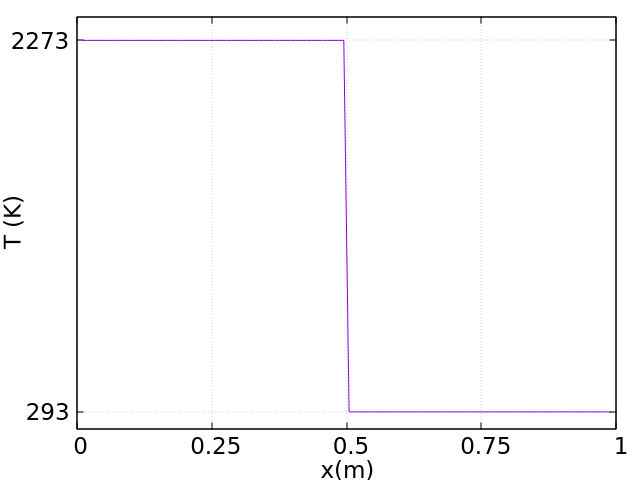
\includegraphics[width=0.3\textwidth]{2000-20step_temp.png}
\captionsetup{font={scriptsize}}
\caption{Temperature profile on the domain}
\label{fig:steptemp}
\end{figure}

\begin{figure}[!h]
\centering
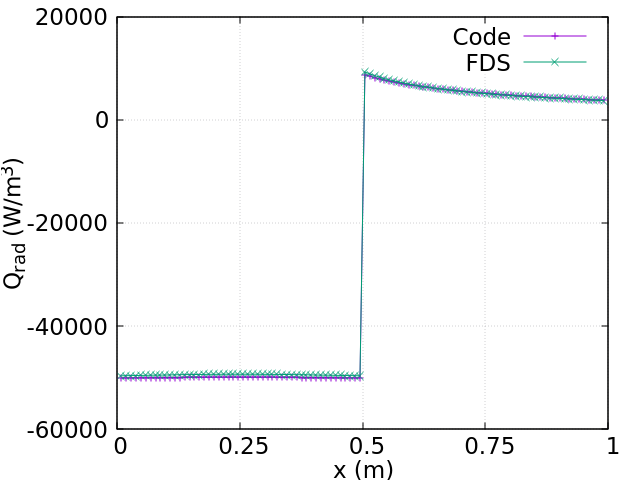
\includegraphics[width=0.3\textwidth]{2000-20step.png}
\captionsetup{font={scriptsize}}
\caption{Comparison between this method and FDS}
\label{fig:stepres}
\end{figure}

\begin{figure}[!h]
\centering
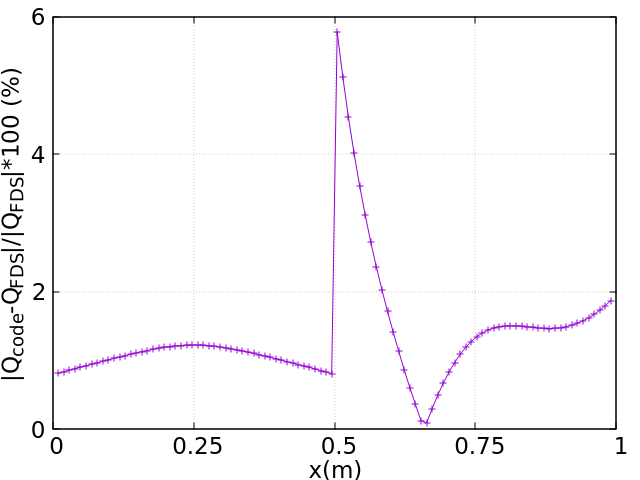
\includegraphics[width=0.3\textwidth]{2000-20step_err.png}
\captionsetup{font={scriptsize}}
\caption{Relative error between this method and FDS}
\label{fig:steprelerr}
\end{figure}

\subsubsection{Multiple Step Case}
That second case is more complex than the previous one because there are consecutive 'steps' in the temperature that can be seen in Fig. \ref{fig:steptemp2}, something like an oscillation. The complexity of the specific case is because, oscillations causes the heat transfer to change direction inside the domain multiple times.
\begin{figure}[!h]
\centering
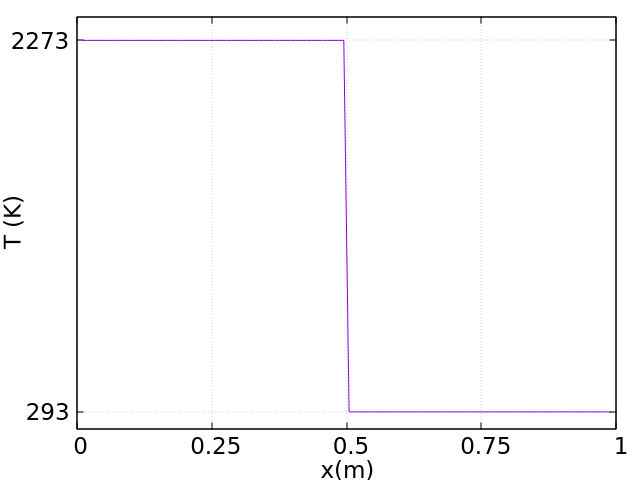
\includegraphics[width=0.3\textwidth]{2000-20step_temp.png}
\captionsetup{font={scriptsize}}
\caption{Temperature profile on the domain}
\label{fig:steptemp2}
\end{figure}

\begin{figure}[!h]
\centering
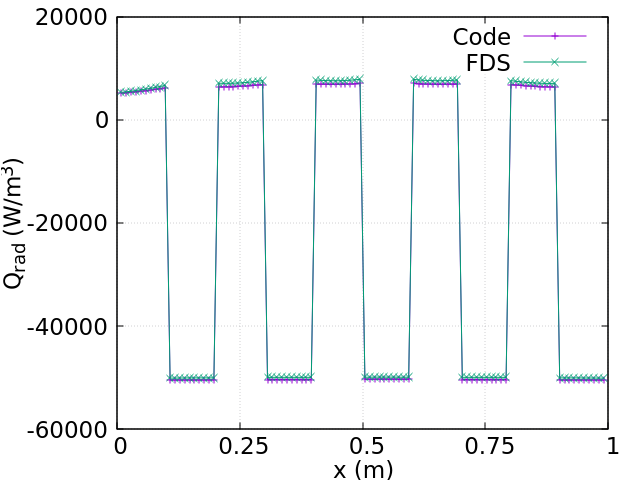
\includegraphics[width=0.3\textwidth]{2000-20mult.png}
\captionsetup{font={scriptsize}}
\caption{Comparison between this method and FDS}
\label{fig:stepres2}
\end{figure}

\begin{figure}[!h]
\centering
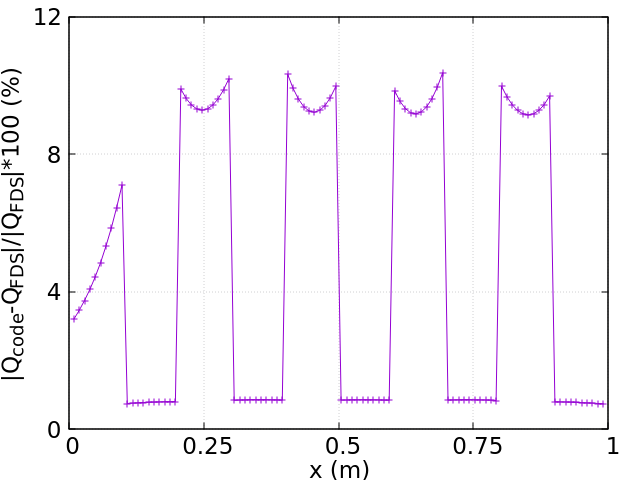
\includegraphics[width=0.3\textwidth]{2000-20mult_err.png}
\captionsetup{font={scriptsize}}
\caption{Relative error between this method and FDS}
\label{fig:steprelerr2}
\end{figure}

\subsubsection{Uniform Temperature}
In that last case a uniform profile of 2000 $^\circ$C was selected in order to check how the code reacts in such situations.
\begin{figure}[!h]
\centering
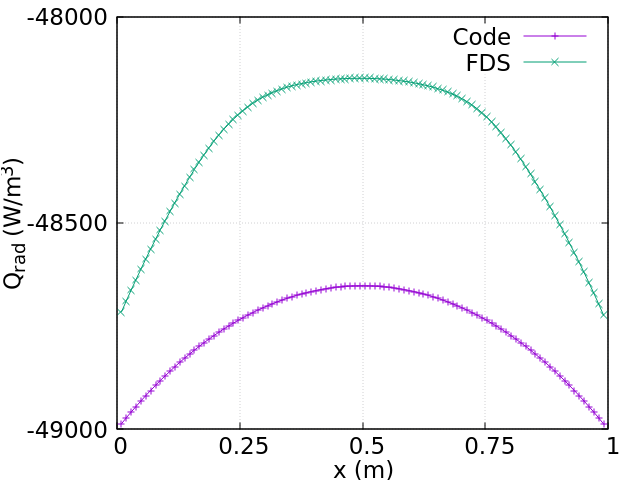
\includegraphics[width=0.3\textwidth]{2000.png}
\captionsetup{font={scriptsize}}
\caption{Comparison between this method and FDS}
\label{fig:unif}
\end{figure}

\begin{figure}[!h]
\centering
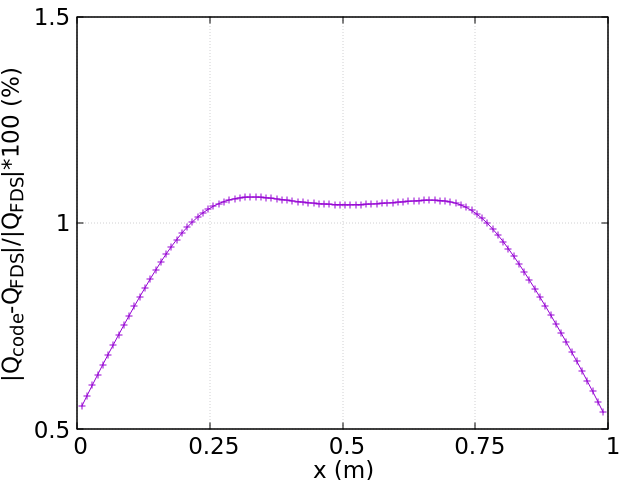
\includegraphics[width=0.3\textwidth]{2000_err.png}
\captionsetup{font={scriptsize}}
\caption{Relative error between this method and FDS}
\label{fig:unifrelerr}
\end{figure}


\section{Fluid Diffusion Model for Radiation Heat Transfer}
\subsection{1-D Fluid Dynamics Equations}
The starting point for deriving this model is the 1-D fluid dynamics equations in Lagrangian mass coordinates \eqref{eq:a}-\eqref{eq:d} where $dr=\rho rdm$ applies. 

\begin{equation}
      \frac{{\partial}r}{\partial t}=U \label{eq:a}
\end{equation}
 
\begin{equation}
    \frac{1}{\rho}=0.5 \frac{{\partial} {r}^2}{\partial m}\label{eq:b}
\end{equation}

\begin{equation}
    \frac{{\partial}U}{\partial t}=-r\frac{{\partial}(\rho+Y)}{\partial m}\label{eq:c}
\end{equation}

\begin{equation}
  \frac{{\partial}\epsilon}{\partial t}+(\rho+Y)\frac{{\partial}\left(\frac{1}{\rho}\right)}{\partial t}=Q  \label{eq:d}
\end{equation}
The system of equations is coupled with the ideal gas law taking the convenient form described at \eqref{eq:idealgas}  .

\begin{equation}
    p=(\gamma-1)\rho\epsilon=\frac{\gamma-1}{\gamma}\rho h\label{eq:idealgas} 
\end{equation}
As far as it concerns the specific internal energy appearing in the energy Eq. above \eqref{eq:d}, an interpolation of experimental data has concluded to a useful function $\epsilon(T,\rho)$ dependent from temperature and density. This function takes the following form $\epsilon=27.7T^{1.5}\left(\frac{\rho}{\rho_0}\right)^{0.12}$. For initial conditions at time $t=0$, an initial channel radius $r_0=0.1\times10^{-2}$ m is set as well as a temperature distribution $T(r,0)=T_0+\frac{T(0,0)}{1+\frac{r^2}{r_0^2}}$ where $T_0=300$ K and $T(0,0)=10^4$ K. The undisturbed air is stationary $U(r,0)=0$ with a constant pressure $p_0=1\text{ atm}=1.01325\times10^5$ Pa and a constant density  $\rho_0=1.17152\text{ kg}/\text{m}^3$.

\subsection{Heat Transfer Modelling}
The non homogeneous part $Q$ of the energy Eq. \eqref{eq:d} plays a major role in this radiation model because it concerns heat influx and heat losses on the flow field. It's also important to notice here that it consists of three terms $ Q=Q_\text{J}+Q_{\lambda}+Q_\text{rad}$. 
\subsubsection{Joule Heating}
The first term \eqref{eq:jouleheat} describes the Joule heating effect Ref. \cite{plooster}, which takes place when an electric current passes through a conductor (i.e. air in our case) and produces heat.
\begin{equation}
    Q_\text{J}=\frac{E^2\sigma}{\rho}\label{eq:jouleheat}
\end{equation}
 For the cases investigated in this work, an aperiodic current pulse leading to a remaining current after discharge of the following form $I=I_\text{a}\cos(2\pi vt)e^{\frac{t}{\tau_a}}+I_\text{res}$  was selected. Due to the electric pulse, the air is ionized and plasma is created. The conductivity of the plasma is given by \eqref{eq:sss} where the electron-ion cross section is given by \eqref{eq:aiav}.
\begin{equation}
    \sigma=\frac{4.173\times10^{-10}(A_1+A_2)T^{-0.5}}{2\times10^{-15}(1-A_1)+A_1a_\text{iav}}\times10^2\label{eq:sss}
\end{equation}

\begin{equation}
    a_\text{iav}=2.8\times10^{-6}T^{-2}
    \left(\frac{A_1+3A_2}{A_1+A_2}\right)^2\log\left(1.727\times10^{-5}\frac{A_1+A_2}{A_1+3A_2}T(A_1\rho )^{-0.5}\right)\label{eq:aiav}
\end{equation}
Finally, the resistance of the channel per unit length is described by \eqref{eq:R} and the developed electric field per unit length following the Ohm's law is $ E=IR$.

\begin{equation}
    R=\frac{1}{\int_{r}2\pi r\sigma dr}\label{eq:R}
\end{equation}

\subsubsection{Heat Transfer by Conduction}
The second term \eqref{eq:conductheat} describes the heating transfer phenomena caused by conduction Ref. \cite{plooster} within the air, a process appearing in the atomic level. It's important to notice here that the ionized air and the created plasma have a serious impact on the way that conduction takes place, that's why we have to take into consideration these effects. 
\begin{equation}
     Q_{\lambda}=-\frac{1}{\rho r}\frac{\partial}{\partial r}\left(rk\frac{{\partial}T}{\partial r}\right)\label{eq:conductheat}
\end{equation}
Thermal conductivity coefficient $k=k_\text{e}+k_\text{r}+k_0$ consists of three terms, in order to include the different processes influencing conduction. Thermal conductivity by electrons is determined by Eq. \eqref{eq:ke} while the contribution from diffusion of recombination energy is given by \eqref{eq:kr} and finally the effect of neutral particles is described by \eqref{eq:k0}

\begin{equation}
     k_\text{e}=0.1488\sigma T\times10^2\label{eq:ke}
\end{equation}

\begin{equation}
    k_\text{r}=2.2\times10^{13}\rho\frac{{\partial}A_0}{\partial T}\times10^2\label{eq:kr}
\end{equation}

\begin{equation}
    k_0=10^3(1-A_1)T^{0.5}\times10^2\label{eq:k0}
\end{equation}
\subsubsection{Heat Transfer by Radiation}
The last heat transfer mechanism included in this model is that of radiation Refs. \cite{shneider,paxton}. Heat transfer by radiation seems to be a very difficult process to model especially in cases where ionized gases appear. That's because properties of ionized gases are not well known functions of frequency and temperature. In this work, the equation for radiation diffusion \eqref{eq:raddif} is solved for three different spectral bands, because a simulation considering the whole spectrum would be very demanding as far as it concerns the computational cost.

\begin{equation}
    \frac{1}{r}\frac{\partial}{\partial r}\left(\frac{r}{3k_\text{v}}\frac{{\partial}U_\text{v}}{\partial r}\right)+k_\text{v}(U_\text{pv}-U_v)=0
    \label{eq:raddif}
\end{equation}
These spectral bands are 0.01-0.52, 6.52-9.96 and 9.96-247 eV and have been chosen after an optimization process. The absorption coefficient $k_v$ is considered to be frequency independent and its value is equal to its median value averaged over the Planck distribution \eqref{eq:bl}
in each band Ref. \cite{avilova,elashevich}. The model used for $k_\text{v}$ \cite{book:zeldovich} \eqref{eq:kv} takes into consideration the different components of air in order to conclude in a final absorption coefficient for the mixture.
\begin{equation}
k_v=\frac{2.56\times10^{12}\frac{T_0P}{TP_0}}{T^2x^3}e^xe^{sp}\times10^2
\label{eq:kv}
\end{equation}
Where $x=\frac{1.44}{\lambda T}$, $\lambda$ the wavelength of the electromagnetic radiation in cm, $P_0=1.01325\times10^5$ Pa and $T_0=300$ K reference pressure and temperature. As far as it concerns the different components of air, the exponent sp can be calculated from the table \ref{tab:1}.

\begin{table}[ht]
    \centering
    \begin{tabular} { | l | l | l | l | l | l | }
 \hline
 Components & $O_2$ & $N_2$ & O & N & NO \\
 \hline
 sp  & $\frac{-140000}{T}$  & $\frac{-181000}{T}$ & $\frac{-158000}{T}$ & $\frac{-169000}{T}$ & $\frac{-108000}{T}$  \\
\hline
\end{tabular}
    \caption{Exponents of $k_v$ model}
    \label{tab:1}
\end{table}
\noindent
Finally, for the mixture of gases the total absorption coefficient can be calculated from the relation \eqref{eq:su}, where $\frac{n_i}{n}$ is the mole fraction and $k_{v_i}$ the absorption coefficient  of the $i^{th}$ component respectively.
\begin{equation}
k_v=\sum_{i=1}^{N}\frac{n_i}{n}k_{v_i} \label{eq:su}
\end{equation}
In Planck's distribution  $k_\text{B}=1.38064\times10^{-23}$ J/K is Boltzman's constant, $h=6.62607\times10^{-34}$ Js is Planck's constant and $c=299722458$ m/s the speed of light.

\begin{equation}
    E=hv \label{eq:pe}
\end{equation}
In Eq. \eqref{eq:raddif} the spectral density of radiation at equilibrium is $U_\text{pv}=\frac{4\pi}{c}B(T,v1,v2
)$ where $v1$ and $v2$ are the lower and upper limits on the frequency domain of the spectral bands and can be found from the Planck-Einstein relation \eqref{eq:pe}. So, these limits of the three spectral bands are $2.418\times10^{12}$-$1.257\times10^{14}$, $1.576\times10^{15}$-$2.408\times10^{15}$ and $2.408\times10^{15}$-$5.973\times10^{16}$ Hz.  



\begin{equation}
    B(T,v1,v2)=\frac{2h}{c^2}\int_{v1}^{v2}\frac{v^3dv }{e^{\frac{hv}{k_B T}}-1} \enspace 
    \label{eq:bl}
\end{equation}
In order to solve the above equation,  a Marshak boundary condition \eqref{eq:mar} was applied at the edge of the computational grid while a Neumann at r=0 \eqref{eq:neum}.

\begin{equation}
    \frac{2}{3k_\text{v}}\frac{{\partial}U_\text{v}}{\partial r}+U_\text{v}=0 \label{eq:mar}
\end{equation}
\begin{equation}
    \frac{{\partial} U_\text{v}}{\partial r}=0 \label{eq:neum}
\end{equation}
After solving numerically the equation, we can determine the heat influx and losses by radiation by using the following relation.

\begin{equation}
    Q_\text{rad}=\frac{c}{\rho}\sum_{sb=1}^3k_\text{v}(U_\text{v}-U_\text{pv})
\end{equation}

\subsection{Numerical Method} 
\subsubsection{Discretization of the Radiation Diffusion Equation}
For the discretization of the radiation diffusion equation, a centered finite difference scheme of second order was selected. By applying the finite difference schemes to the  equation, we conclude to the discretized equation, where $U_\text{v}$ was replaced by $U$.

\begin{equation}
    \left.\frac{r}{k_v}\right\vert_{i+\frac{1}{2}}\frac{U_{i+1}-U_{i}}{dr^2}-\left.\frac{r}{k_v}\right\vert_{i-\frac{1}{2}}\frac{U_{i}-U_{i-1}}{dr^2}-3k_vr_iU_i+3k_vr_iU_{\text{pv}_i}=0 \label{eq:disc1}
\end{equation}
Where $r_{i+\frac{1}{2}}=r_i+\frac{dr}{2}$, $r_{i-\frac{1}{2}}=r_i-\frac{dr}{2}$ while for the calculation of $k_{v_{i+\frac{1}{2}}}$ and $k_{v_{i-\frac{1}{2}}}$ the temperature and the pressure as a mean value of these at the cells $i$, $i+1$ and $i$, $i-1$ respectively is used.
As far as it concerns the boundary conditions, at the edge of the computational domain they will take the following form \eqref{eq:bc1}.

\begin{equation}
\frac{U_2-U_1}{dr}=0,\enspace \frac{2}{3k_{v_n}}\frac{U_n-U_{n-1}}{dr}+U_n=0 \label{eq:bc1}
\end{equation}

\subsubsection{Integration of the Radiation Diffusion Equation }
For the integration of the discretized equation, we have to rearrange the terms and set the known quantity $A_i=\left.\frac{r}{k_{v}}\right\vert_i$ for our convenience. After these operations, we conclude to a convenient form of the discretized radiation diffusion Eq. which is the following \eqref{eq:disc2}.

\begin{equation}
    A_{i-\frac{1}{2}}U_{i-1}+\left(-A_{i-\frac{1}{2}}-A_{i+\frac{1}{2}}-3r_idr^2k_{v_i}\right)U_i+A_{i+\frac{1}{2}}U_{i+1}=-3r_ik_{v_i}dr^2U_{\text{pv}_i}\label{eq:disc2}
\end{equation}
The above form of the equation accompanied with the discretized boundary conditions, is a linear system of equations of the form $a_{i-1}x_{i-1}+b_ix_i+c_{i+1}x_{i+1}=d_i$ with only unknown the quantity $x_i=U_i$ at each cell of the computational domain. This system of equations can be solved by using the numerical algorithm TDMA which is a modification of the Gauss elimination method and takes advantage of the three diagonals domination in order to solve the system faster. First of all, this algorithm modifies the known coefficients into a more convenient form as shown at \eqref{eq:coef} and then the final solution of the system can be obtained by the back substitution process as shown at \eqref{eq:bs} . 


\begingroup
\large
\begin{equation}
\displaystyle c_i' = \begin{cases} 
      \frac{c_i}{b_i} & \text{:\enspace $i=1$} \\
      \frac{c_i}{bi-a_ic_{i-1}'} & \text{:\enspace $i=2,3,...,n-1$} \\ 
   \end{cases}
   \displaystyle \enspace d_i' = \begin{cases}
      \frac{d_i}{b_i} & \text{:\enspace $i=1$} \\
      \frac{d_i-a_id_{i-1}'}{bi-a_ic_{i-1}'} & \text{:\enspace $i=2,3,...,n-1$} \\
   \end{cases}
   \label{eq:coef}
\end{equation}
\endgroup

\vspace{10mm}

\begingroup
\large
\begin{equation}
\begin{cases} 
     x_n=d_n \\
     x_i=d_i'-c_i'x_{i+1} & \text{:\enspace $i=n-1,n-2,...,1$} \\
   \end{cases}
      \label{eq:bs}
\end{equation}
\endgroup
In order to check the rate of convergence of the above process, we have to calculate the residual \eqref{eq:res}. The residual is the sum  of all discretized source terms and discretized derivatives and shows whether the equation is finally satisfied after the numerical method has ended. In order to do that, we calculate the maximum residual in the computational domain and if it has a value close to zero, it proves that the radiation diffusion equation is solved correctly. 

\begin{equation}
  R=A_{i-\frac{1}{2}}U_{i-1}+\left(-A_{i-\frac{1}{2}}-A_{i+\frac{1}{2}}-3r_idr^2k_{v_i}\right)U_i+A_{i+\frac{1}{2}}U_{i+1}+3r_ik_{v_i}dr^2U_{\text{pv}_i}\label{eq:res}
\end{equation}

\subsection{Validation of the Code}
The next step is to validate our code and for this purpose, data form Ref. \cite{shneider} were used. As this code is steady state and can't take into consideration the time evolution of the described phenomena, data on a specific time have to be used. The case that was selected for validation is that of $t=0.1\mu s$. Also, as this code doesn't solve the hydrodynamic flow field but takes as inputs the distributions of temperature and density, these information have to be digitized and interpolated on the grid created by the code in order to solve the radiation diffusion equation. The distributions presented below Figs. \ref{fig:rho}, \ref{fig:T} are the exact inputs of the code.

\begin{figure}[!h]
\centering
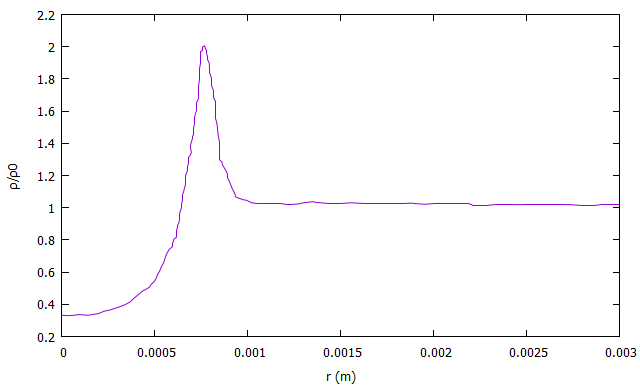
\includegraphics[width=0.52\textwidth]{rho.png}
\captionsetup{font={scriptsize}}
\caption{Dimensionless density distribution on the domain}
\label{fig:rho}
\end{figure}
\begin{figure}[!h]
\centering
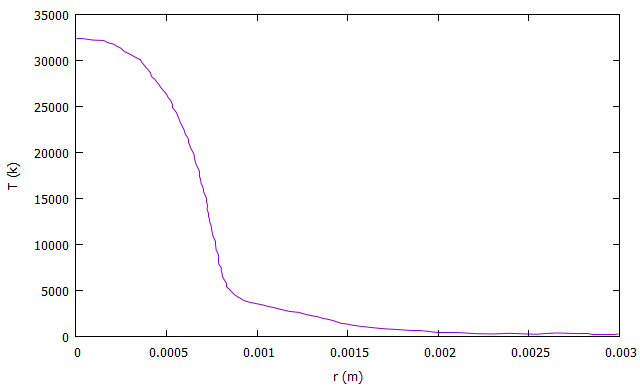
\includegraphics[width=0.52\textwidth]{T.png}
\captionsetup{font={scriptsize}}
\caption{Temperature distribution on the domain}
\label{fig:T}
\end{figure}

\vspace{150mm}




  

\bibliographystyle{warpdoc}
 \bibliography{all}
\end{document}





